\section{Results}   \label{sec:Results}

In this section, I first present the algorithm I developed, to return the optimal credit card portfolio, given a set of user variables and card parameters.
I then describe the results of a sensitivity analysis and Monte Carlo simulation that show how the return on spend and marginal benefit depend on the user variables.
Finally, I will describe the interactive \sR\ \textsf{Shiny} app that is available online for people to play with and to get a recommended credit card portfolio tailored to their personal preferences. 

\subsection{Portfolio Recommendation Algorithm}

The model described in Sections \ref{sec:Theory} and \ref{sec:Specification} is coded in \sR\ using two functions that are saved in the file \texttt{CCPortfolioFunctions.R}.
The function \texttt{get\_budget(income, budget\_data)} is a helper function that returns the budget as a named vector, given a gross income, corresponding to the 18 credit card categories from Sect.~\ref{subsec:CreditCardData} and using the BLS CES income-dependent data described in Sect.~\ref{subsec:UserData}.
This budget is then used as input for the second function, \texttt{get\_portfolio(K, eta, theta, cards\_data, budget, verbose = TRUE)}, which returns a named list with the optimized portfolio of credit cards, as well as some other useful metrics (the total net benefit in dollars, percentage return on spend, the marginal benefit in dollars per card, the total spend, and which card to use for each spending category). 
The full code of both these functions is presented in the Code Appendix on page~\pageref{app:Code}. 

\begin{figure}[tbh]
    \begin{center}
    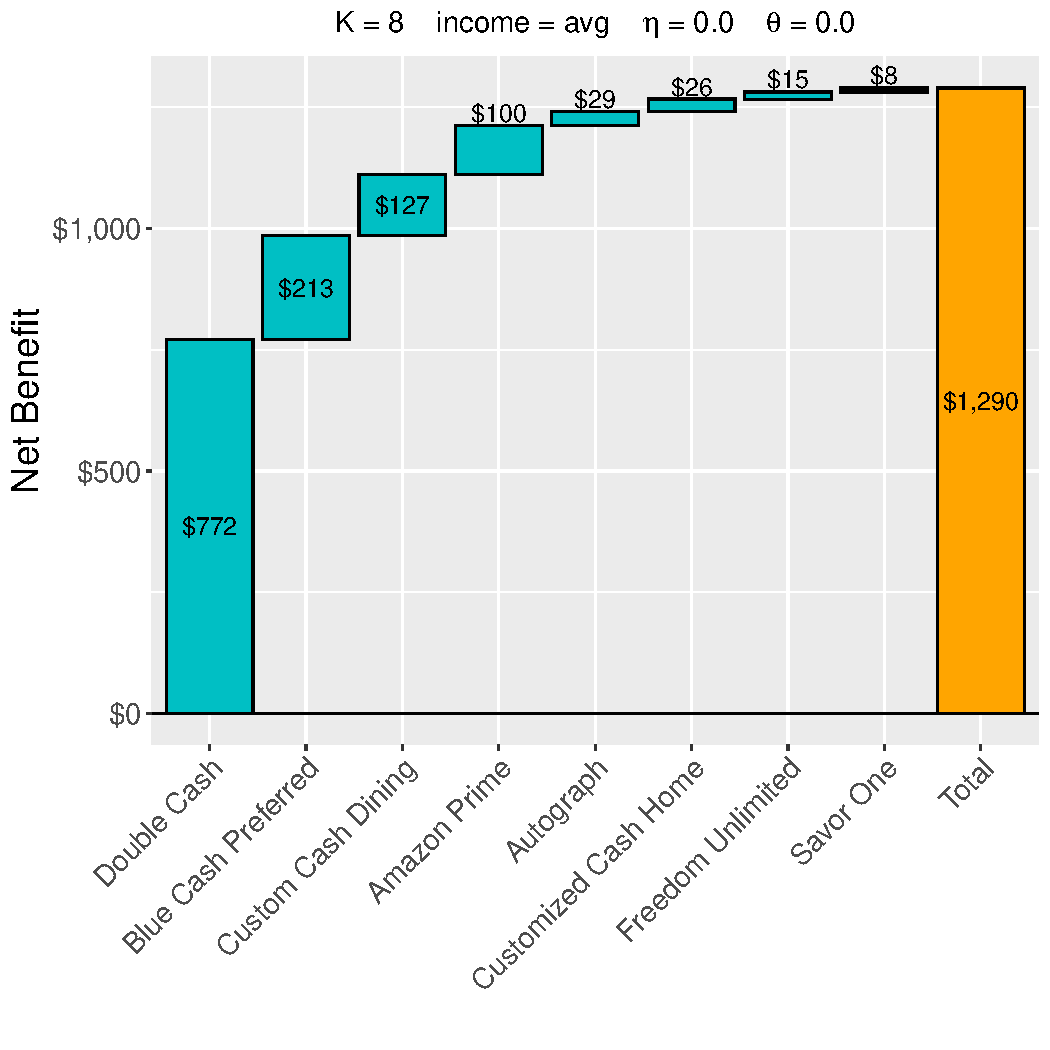
\includegraphics[width=0.6\textwidth]{../Figures/Waterfall_avg_8_0_0.pdf}
    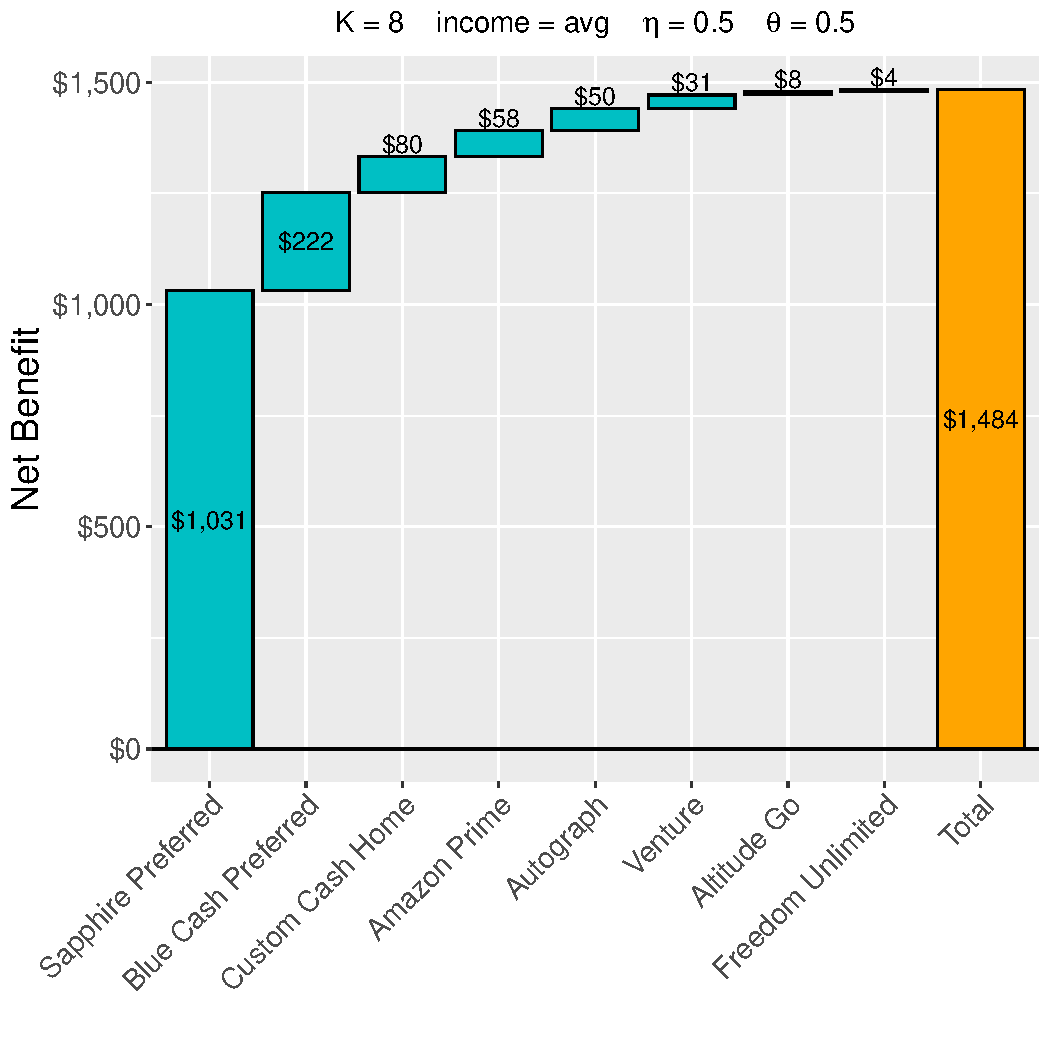
\includegraphics[width=0.6\textwidth]{../Figures/Waterfall_avg_8_05_05.pdf}
    \caption{Waterfall-style summary of two recommended portfolios, for different user preferences. Both figures returned the best 8 cards ($K=8$) for the budget of the average consumer (income $=$ avg). The first card is on the left and the bars indicate the marginal benefit of adding each additional card. The top panel user has a cashback preference and uses no static benefits ($\eta$ and $\theta$ both equal 0). The bottom panel user transfers half the points to travel partners ($\eta = 0.5$) and uses half of each card's benefits ($\theta = 0.5$).}
    \label{fig:Waterfall}
    \end{center}
\end{figure}

Figure~\ref{fig:Waterfall} summarizes some of the algorithm's essential output in a user-friendly format, for two different user preferences. 
The figure shows that the algorithm is successful in recommending different portfolios for different users. 
The more cashback-oriented user (top panel) gets recommended more cashback focused cards, while the more travel-oriented user (bottom panel) gets recommended a few more travel focused cards, which results in a higher total benefit (the orange bar on the right).
Note that the marginal benefit plotted per card is the \emph{additional} benefit that the card delivers, \emph{on top} of the cards already selected to its left.  
In other words, this marginal benefit includes the opportunity cost of taking spend categories away from the cards to its left, in order to put that spend on the additional card. 

Figure~\ref{fig:Waterfall} also shows that the marginal benefit diminishes with more cards, which is by design of the greedy algorithm. 
The algorithm will always recommend cards with the highest marginal benefit first. 
It is up to the user of the recommendation app (see Sect.~\ref{subsec:ShinyApp}) to decide at which marginal benefit it is no longer worth it to add additional cards, but for the remainder of this paper I assume that \$50 is probably a reasonable amount for most people to stop adding to the portfolio. 
This allows me to determine the ``sweet spot'' for the credit card portfolio size, as a function of the variables. 
I discuss this sweet spot, along with some other metrics of the recommended portfolios, in the next section.

\clearpage
\subsection{Sensitivity Analysis}

Figures \ref{fig:MBvsKvsIncome_0_0}, \ref{fig:MBvsKvsIncome_05_05}, and \ref{fig:MBvsKvsIncome_1_1} show the marginal benefit as a function of the number of cards, for different incomes, and for $(\eta, \theta)$ equal to $(0,0)$, $(0.5,0.5)$, and $(1,1)$, respectively.
The income levels for these figures are chosen to represent the average incomes of the nine income levels of the BLS CES data (Table~\ref{tab:BudgetIncome} in the Data Appendix), while the thick black dashed line represents the average budget of all consumers in the survey (with an average income of \$94k).
These figures show that for most people, regardless of preferences or income, four or five is the sweet spot for the number of credit cards to hold, before the additional benefit drops below \$50.  
There seems to be some evidence that the highest three income levels (above $\$100,000$) maintain a higher marginal benefit with more cards (up to six or seven, before the benefit drops below \$50).

\begin{figure}[tbh]
    \begin{center}
    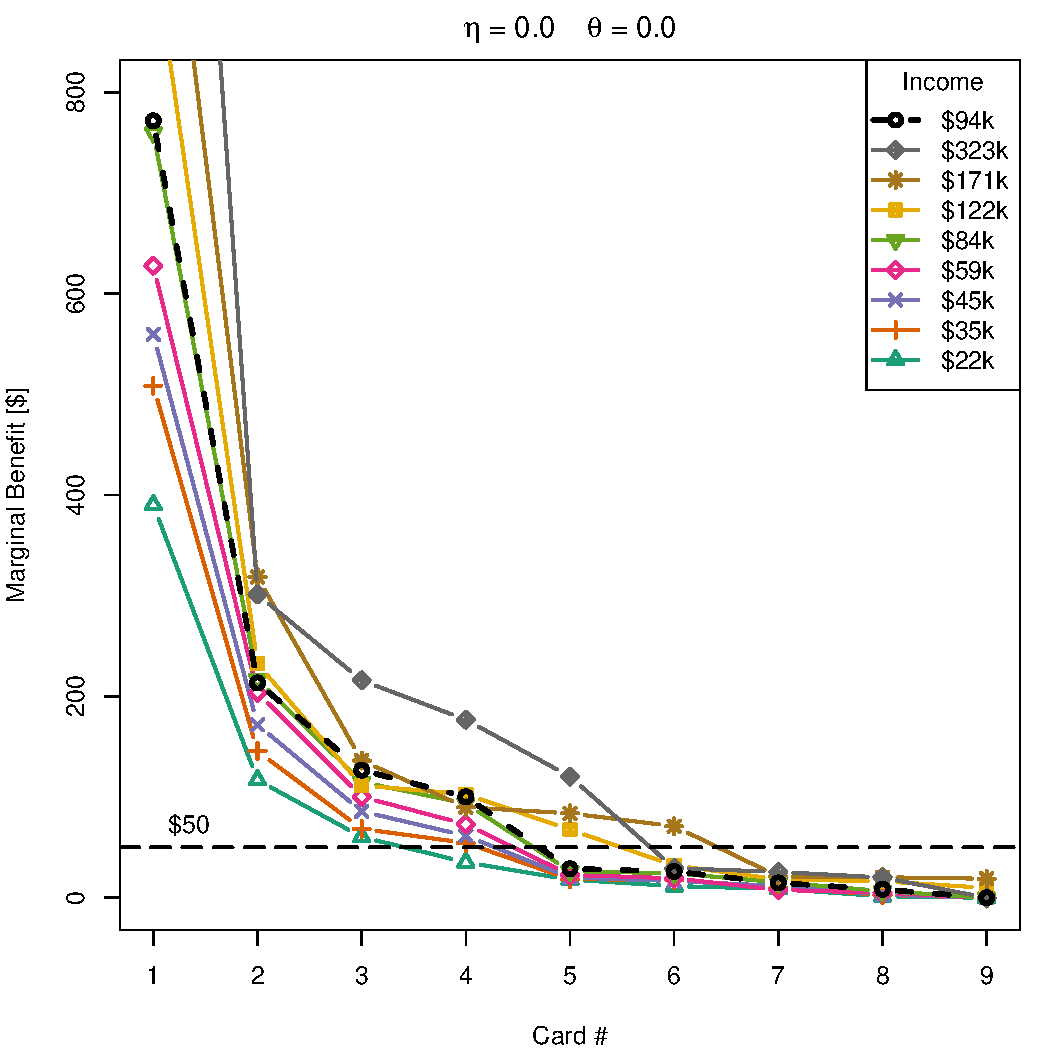
\includegraphics[width=0.6\textwidth]{../Figures/MBvsKvsIncome_0_0.pdf}
    \caption{Marginal benefit versus number of cards, assuming $(\eta, \theta) = (0,0)$.}
    \label{fig:MBvsKvsIncome_0_0}
    \end{center}
\end{figure}

\begin{figure}[tbh]
    \begin{center}
    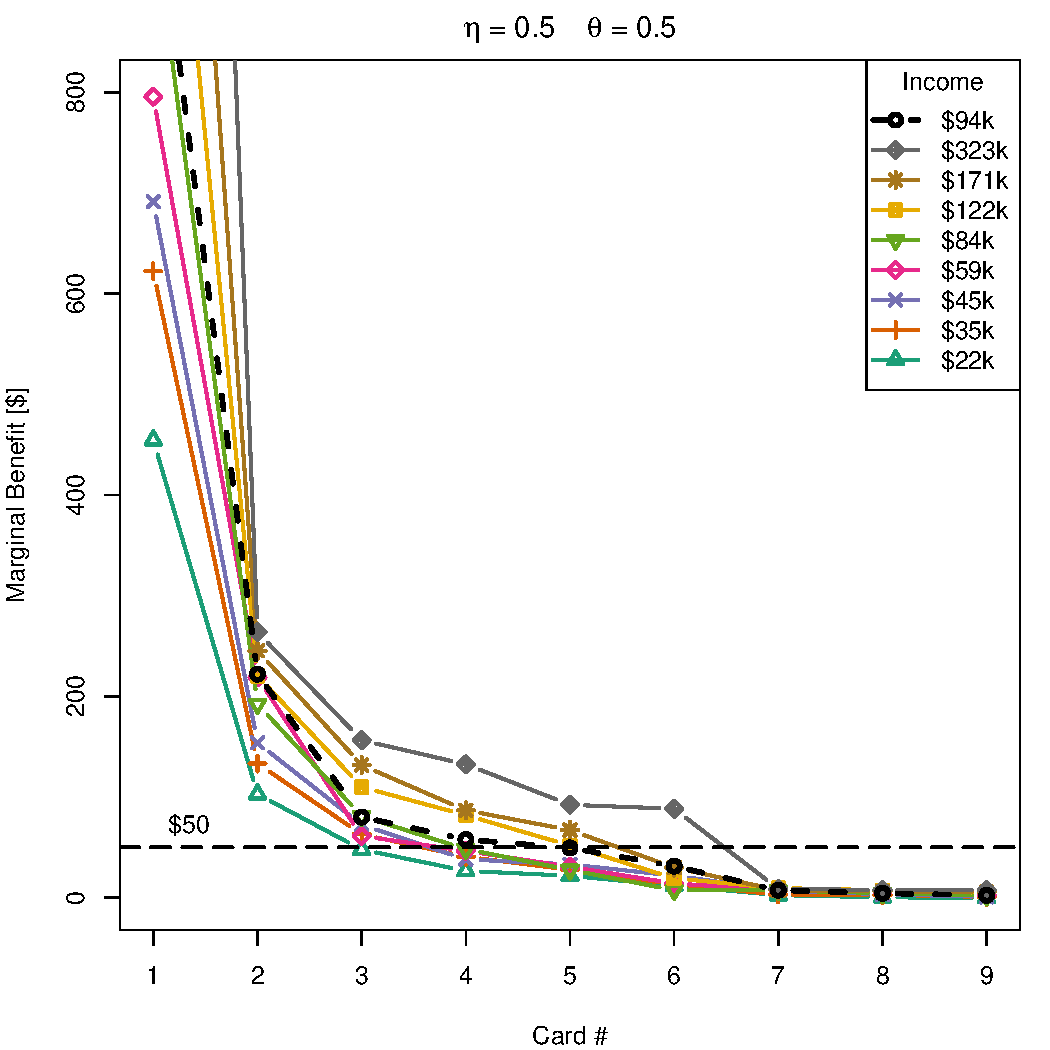
\includegraphics[width=0.6\textwidth]{../Figures/MBvsKvsIncome_05_05.pdf}
    \caption{Marginal benefit versus number of cards, assuming $(\eta, \theta) = (0.5,0.5)$.}
    \label{fig:MBvsKvsIncome_05_05}
    \end{center}
\end{figure}

\begin{figure}[tbh]
    \begin{center}
    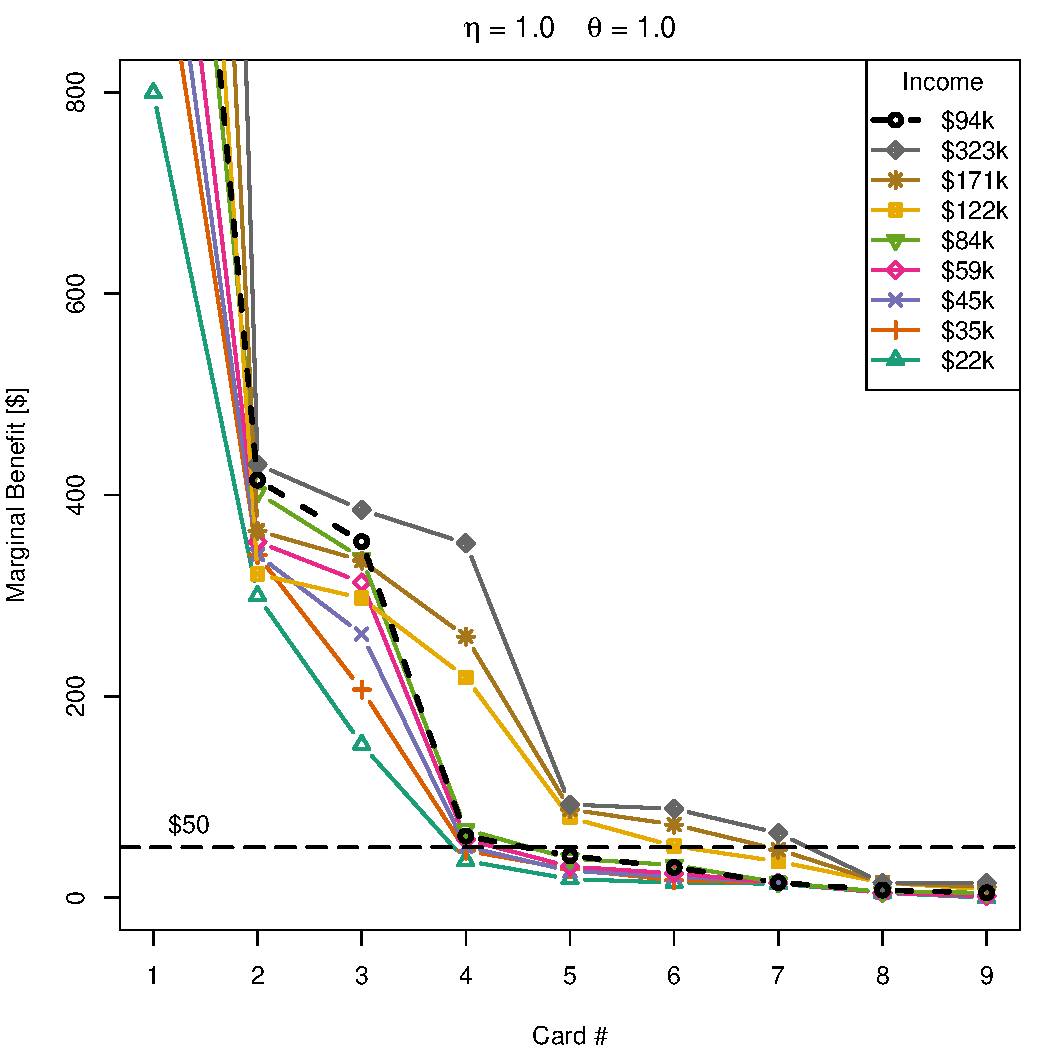
\includegraphics[width=0.6\textwidth]{../Figures/MBvsKvsIncome_1_1.pdf}
    \caption{Marginal benefit versus number of cards, assuming $(\eta, \theta) = (1,1)$.}
    \label{fig:MBvsKvsIncome_1_1}
    \end{center}
\end{figure}

Figures \ref{fig:ROSvsKvsIncome_0_0}, \ref{fig:ROSvsKvsIncome_05_05}, and \ref{fig:ROSvsKvsIncome_1_1} show the total return on spend versus the number of cards, for the same choice of $(\eta, \theta)$ as the previous three figures. 
These figures show that ROS converges to $\sim3.2$ percent for cashback-oriented users, regardless of income level (Fig.~\ref{fig:ROSvsKvsIncome_0_0}).
Once travel transfer partners and benefits are being used, Figs.~\ref{fig:ROSvsKvsIncome_05_05} and~\ref{fig:ROSvsKvsIncome_1_1} show that there is more variation among different income levels. 
As expected, travel and benefits return additional value, and increase ROS for all incomes.
Once all benefits are being used, however ($\theta = 1$, Fig.~\ref{fig:ROSvsKvsIncome_1_1}), we see an interesting reversal in the effect for different incomes: the lowest income levels reach a ROS comparable, or even higher, than the highest income levels (e.g., note the cyan triangles above the gray diamonds). 
Consumers at the lowest income levels can spend much less on credit cards compared to high-income consumers, but Fig.~\ref{fig:ROSvsKvsIncome_1_1} reminds us that low-income consumers can benefit more, relative to their spend, as long as they make full use of the static credit card benefits.
Figure~\ref{fig:ROSvsKvsIncome_1_1} also shows that 5.5--6.5 percent is roughly the maximum ROS people can expect, when making full use of an optimized portfolio of 4--5 credit cards.
 
\begin{figure}[tbh]
    \begin{center}
    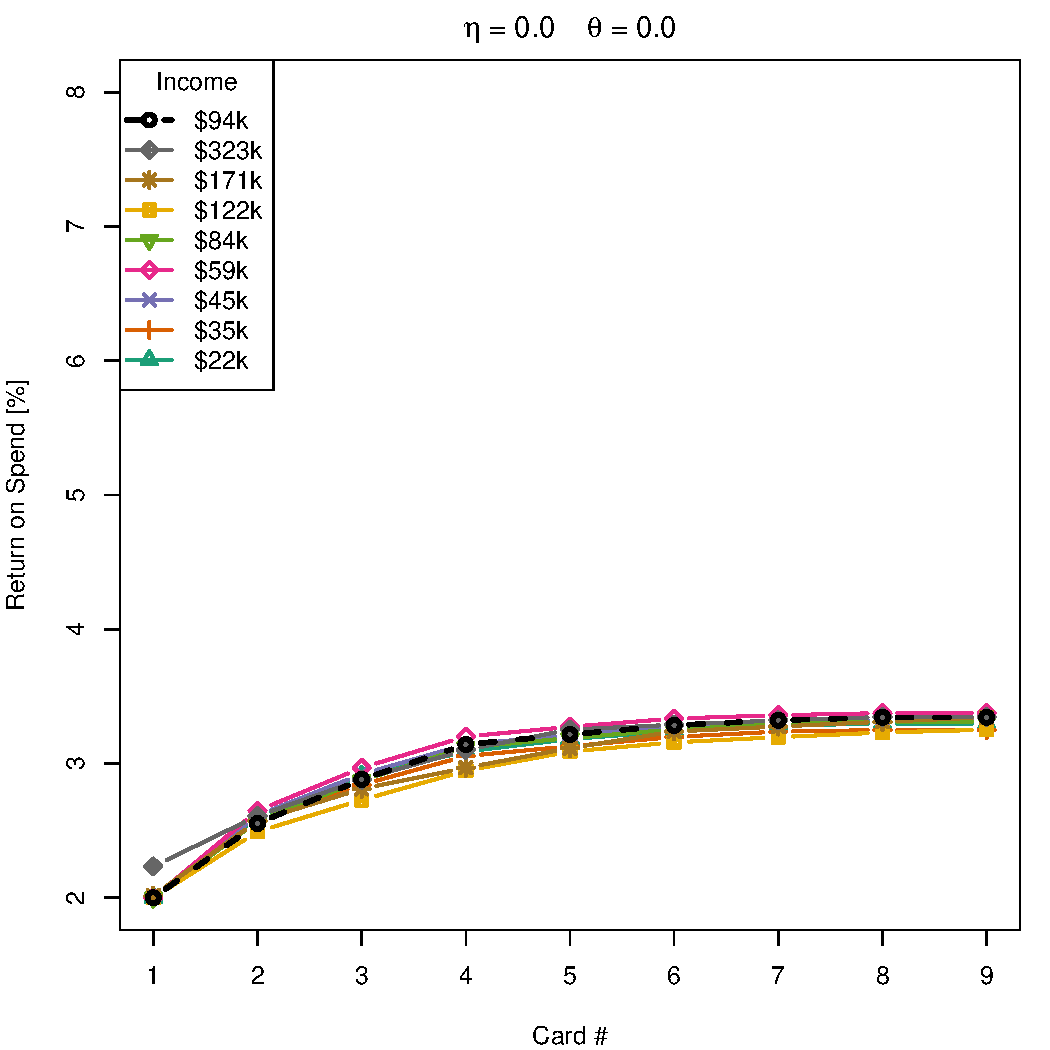
\includegraphics[width=0.6\textwidth]{../Figures/ROSvsKvsIncome_0_0.pdf}
    \caption{Total return on spend versus the number of cards, assuming $(\eta, \theta) = (0,0)$.}
    \label{fig:ROSvsKvsIncome_0_0}
    \end{center}
\end{figure}

\begin{figure}[tbh]
    \begin{center}
    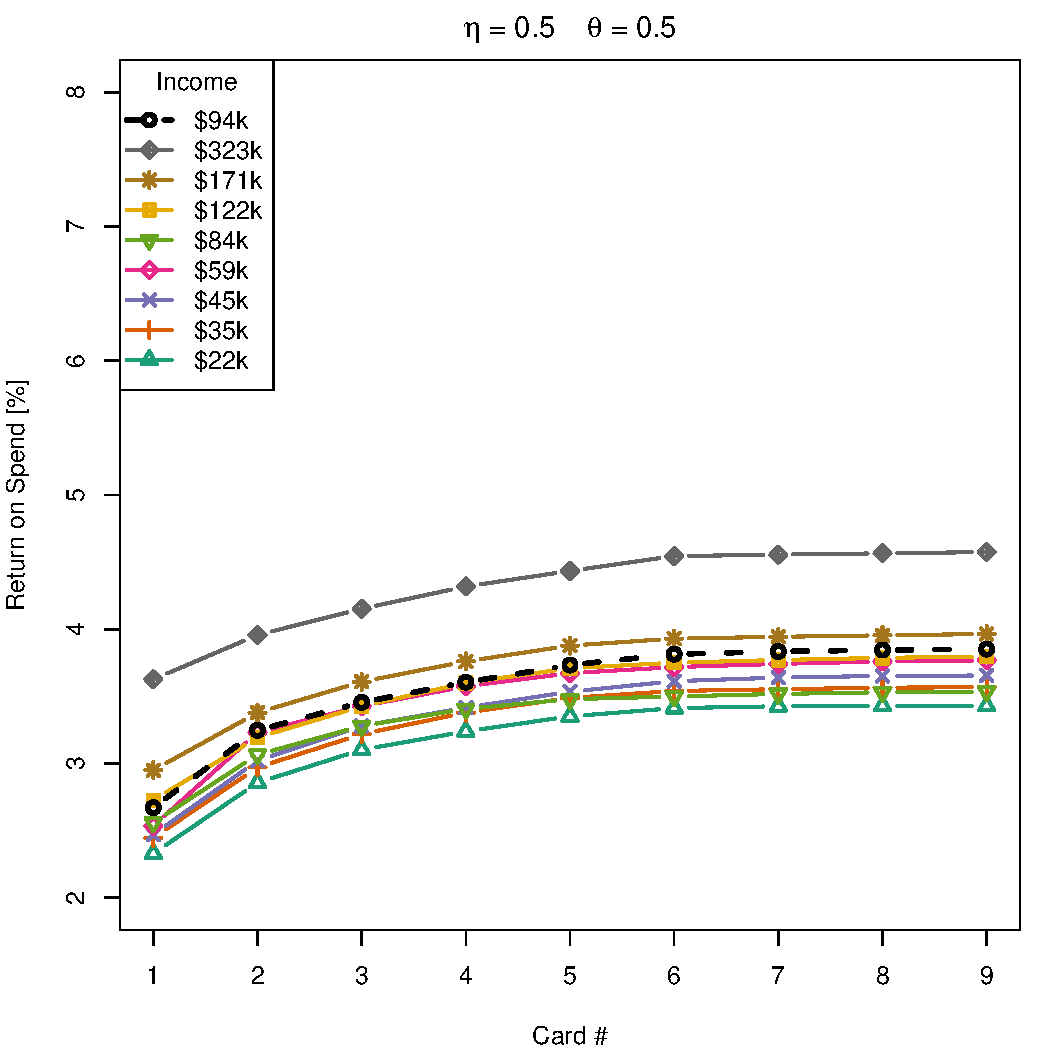
\includegraphics[width=0.6\textwidth]{../Figures/ROSvsKvsIncome_05_05.pdf}
    \caption{Total return on spend versus the number of cards, assuming $(\eta, \theta) = (0.5,0.5)$.}
    \label{fig:ROSvsKvsIncome_05_05}
    \end{center}
\end{figure}

\begin{figure}[tbh]
    \begin{center}
    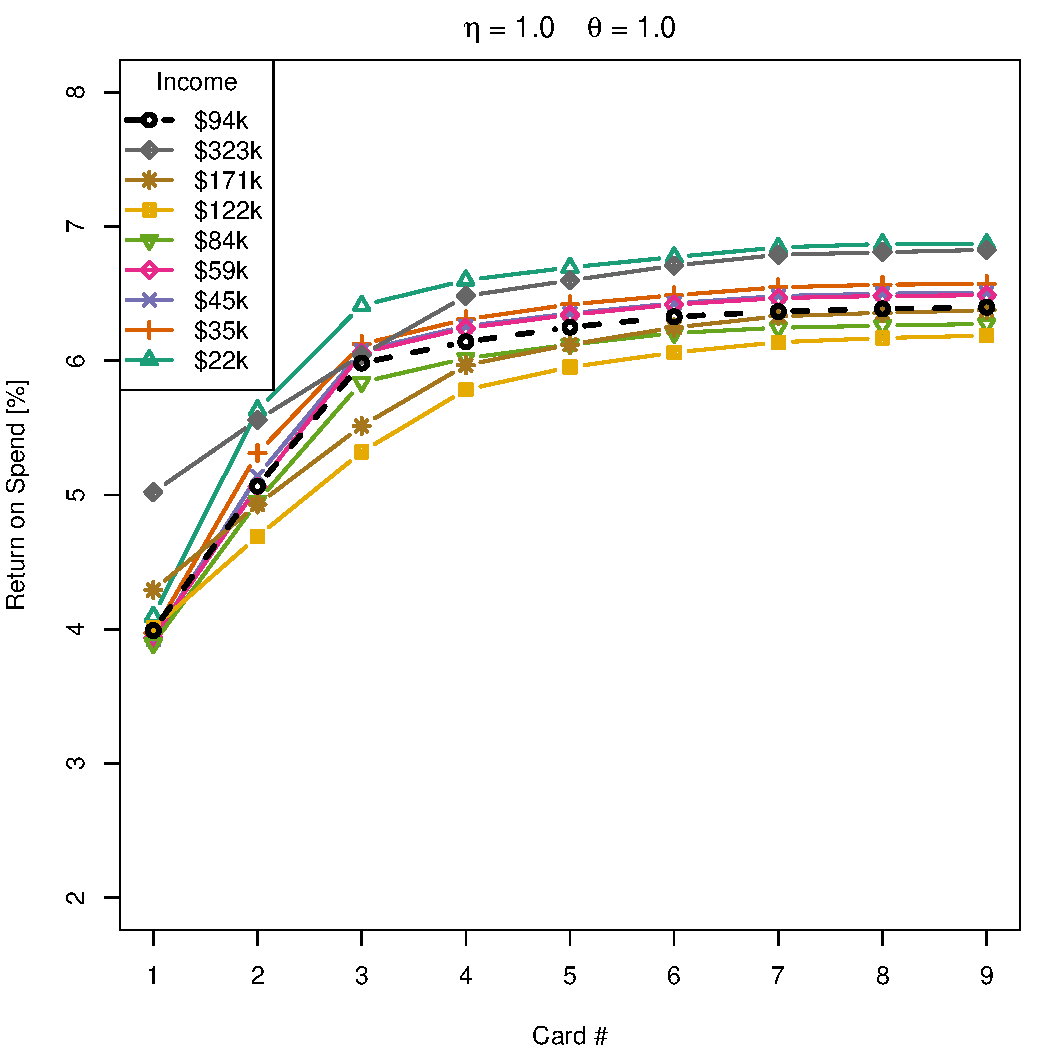
\includegraphics[width=0.6\textwidth]{../Figures/ROSvsKvsIncome_1_1.pdf}
    \caption{Total return on spend versus the number of cards, assuming $(\eta, \theta) = (1,1)$.}
    \label{fig:ROSvsKvsIncome_1_1}
    \end{center}
\end{figure}

Figure~\ref{fig:NBvsIncome} shows the range in total net benefit (in dollars) versus income.  
This range lies between $\sim\$700$--$\$1200$ for the lowest incomes, and increases all the way up to $\sim\$2000$--$\$5000$ for incomes above \$300k.

\begin{figure}[t!bh]
    \begin{center}
    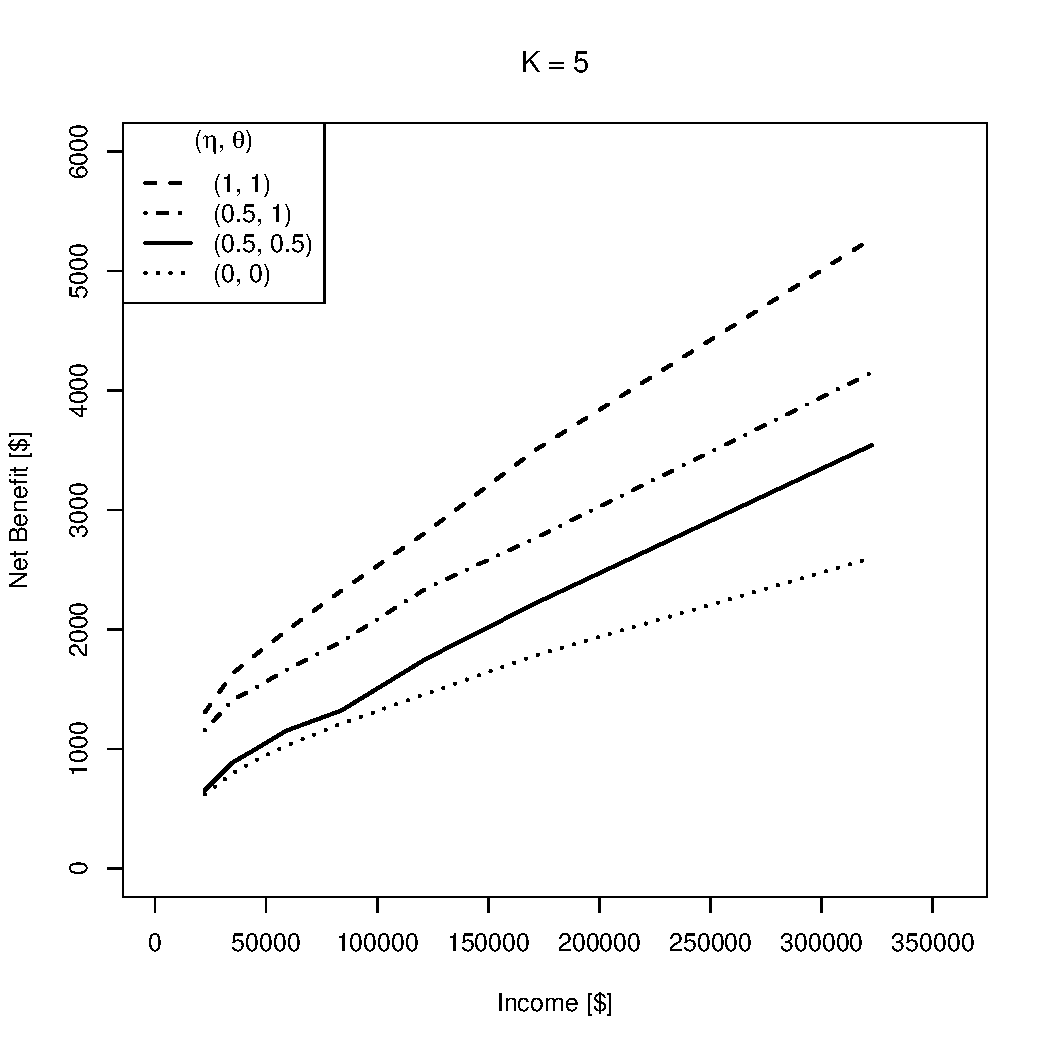
\includegraphics[width=0.6\textwidth]{../Figures/NBvsIncome_K5.pdf}
    \caption{The total net benefit versus income for different combinations of $\eta$ and $\theta$. }
    \label{fig:NBvsIncome}
    \end{center}
\end{figure}

\clearpage
\subsection{Monte Carlo Simulation}

Above we have seen how income and user preferences impact the expected return on spend from rewards credit cards.
Income affects these results in two ways, as can be seen from Table~\ref{tab:BudgetIncome} in the Data Appendix.
First of all, total spend scales with income; higher incomes can spend more on credit cards, although the total spend as a fraction of income goes down (i.e., higher incomes can put more money toward savings and housing, which does not end up on credit cards).
Second, with changing incomes there are also shifts in the spending budgets; essential goods like groceries and gas form a much larger part of the budget for lower incomes, compared to higher incomes. 

To represent more accurately how these patterns affect the benefits of rewards credit cards for a large group of users, I performed a Monte Carlo simulation using 100,000 samples. 
The family income distribution of 57,005 Floridians was used, as described in Sect.~\ref{sec:Data} and presented in Fig.~\ref{fig:IncomeDistribution}.
This distribution was sampled, with replacement, 100,000 times, and for each income the  average budget from the corresponding income bin from the BLS CES data was assumed. 
Each income was then combined with a random value for $K$ (between 1--8), $\eta$ (0--1), and $\theta$ (0--1), which were sampled from uniform distributions.
The optimal portfolio was determined for each sample, and results regarding net benefits, return on spend, and a count of each selected credit card was saved to a \texttt{.csv} file for further analysis. 
This simulation took roughly two hours to process on a 2023 MacBook Pro.

\begin{figure}[t!bh]
    \begin{center}
    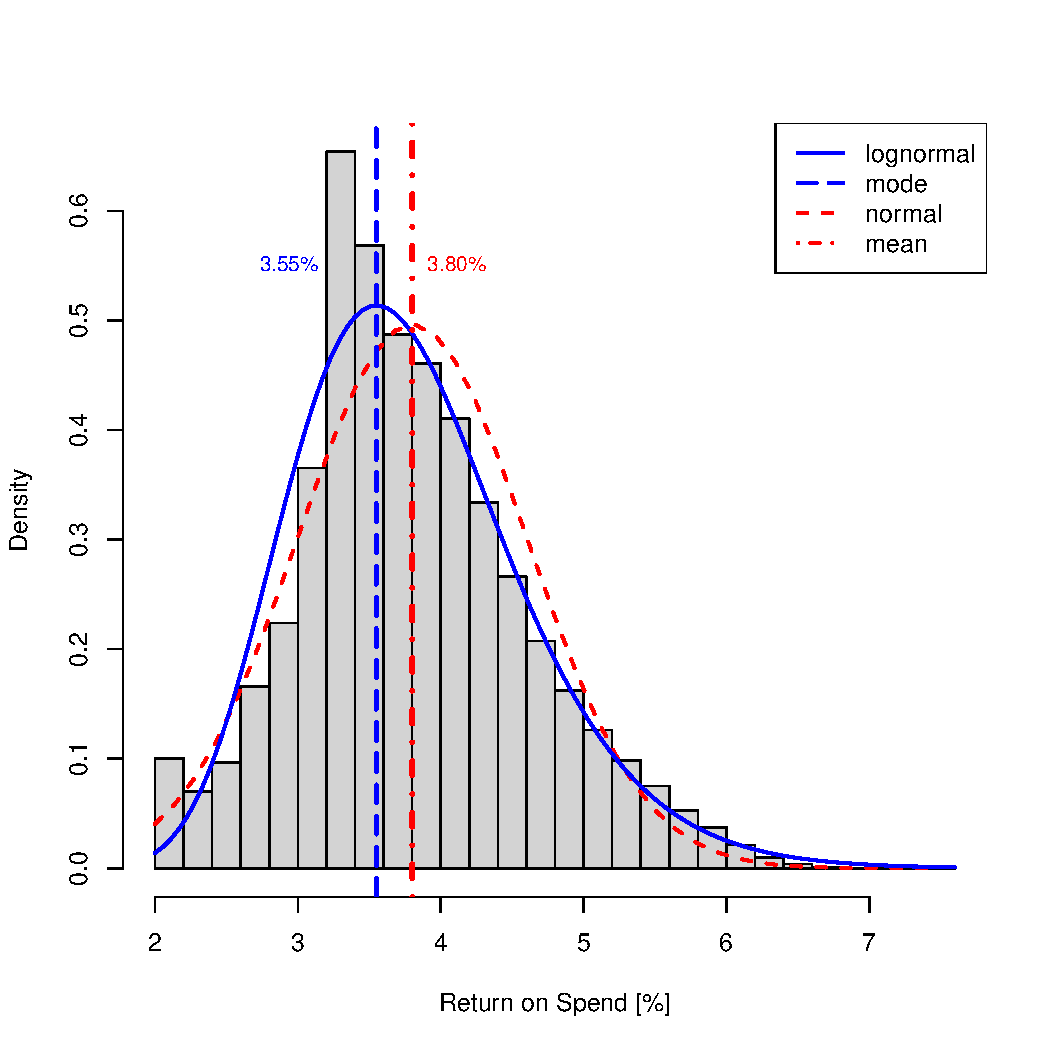
\includegraphics[width=0.6\textwidth]{../Figures/MC_ROS_Histogram.pdf}
    \caption{Distribution of return on spend, resulting from the Monte Carlo simulation.}
    \label{fig:MC_ROS_Histogram}
    \end{center}
\end{figure}

Figure~\ref{fig:MC_ROS_Histogram} shows the ROS distribution resulting from the Monte Carlo simulation.
The distribution approximates a lognormal with a mode at 3.55~percent, while the mean ROS is 3.80~percent with a standard deviation of 0.80.

\begin{figure}[t!bh]
    \begin{center}
    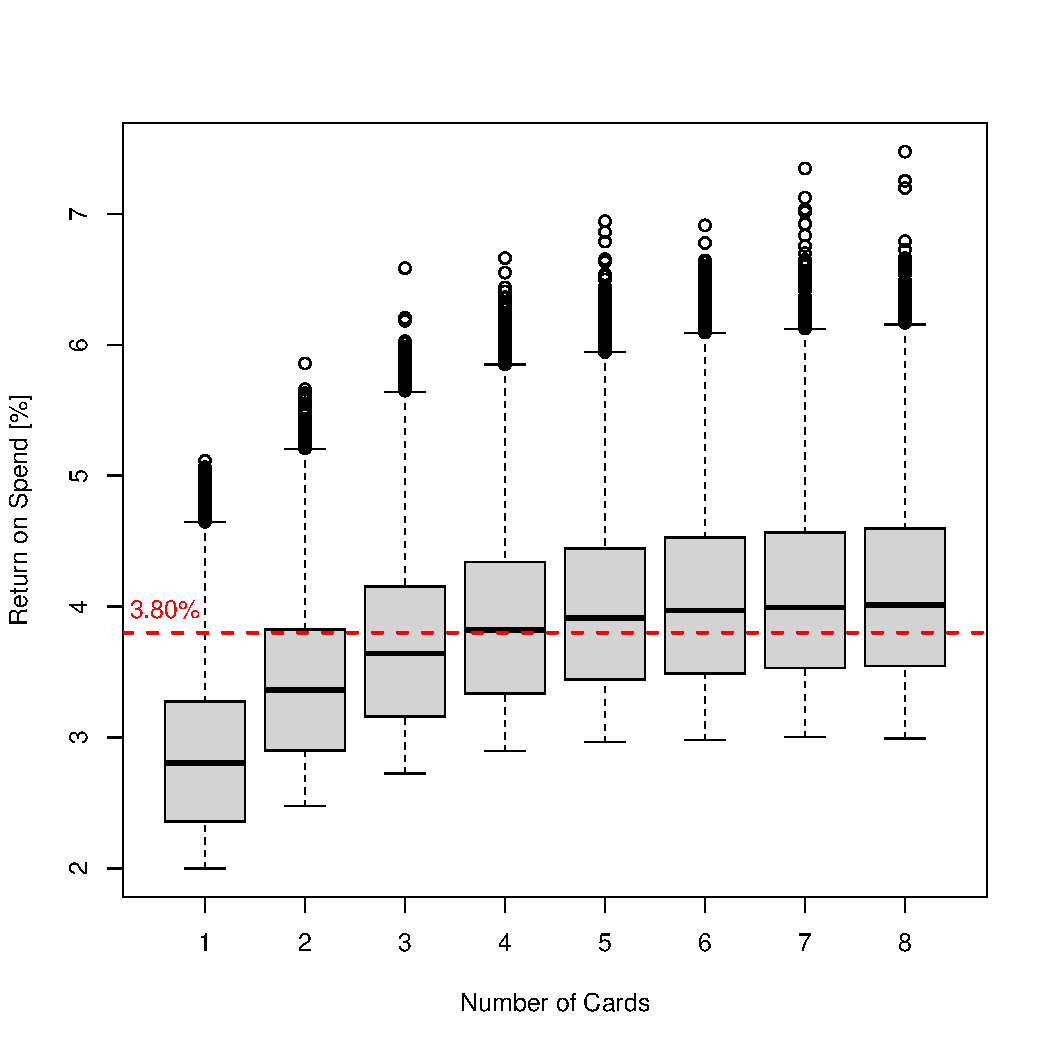
\includegraphics[width=0.6\textwidth]{../Figures/MC_ROS_vs_K.pdf}
    \caption{Boxplot of the return on spend versus the number of cards, resulting from the Monte Carlo simulation. The horizontal dashed line indicates the mean ROS of 3.80~percent, which is very close to the mean ROS of consumers using four credit cards.}
    \label{fig:MC_ROS_vs_K}
    \end{center}
\end{figure}

Figure~\ref{fig:MC_ROS_vs_K} shows a boxplot of the return on spend versus the number of cards, which confirms the earlier observations that marginal benefit diminishes strongly after four or five cards.

\begin{figure}[t!bh]
    \begin{center}
    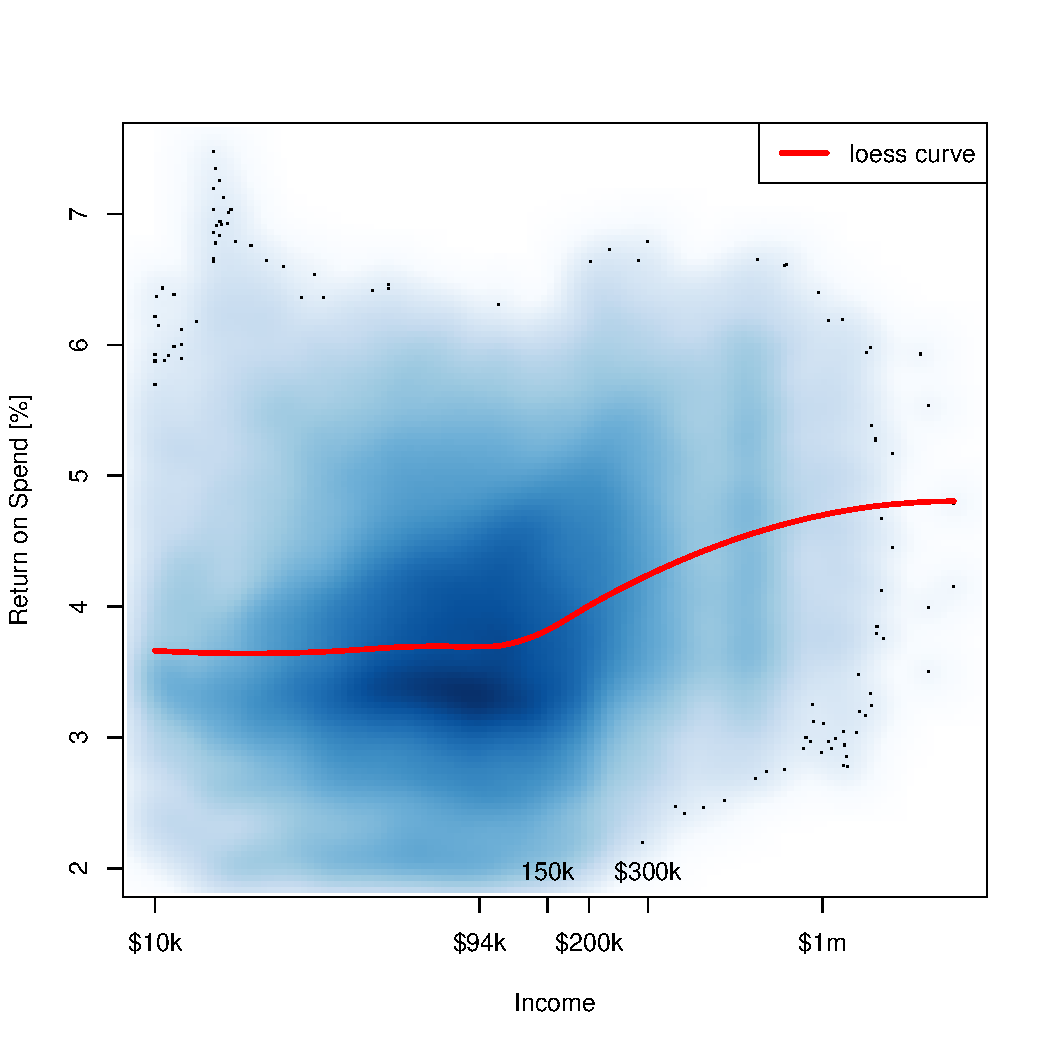
\includegraphics[width=0.6\textwidth]{../Figures/MC_ROS_vs_Income.pdf}
    \caption{Smoothed density scatterplot of return on spend versus income, for all 100,000 simulated portfolios.}
    \label{fig:MC_ROS_vs_Income}
    \end{center}
\end{figure}

\begin{figure}[t!bh]
    \begin{center}
    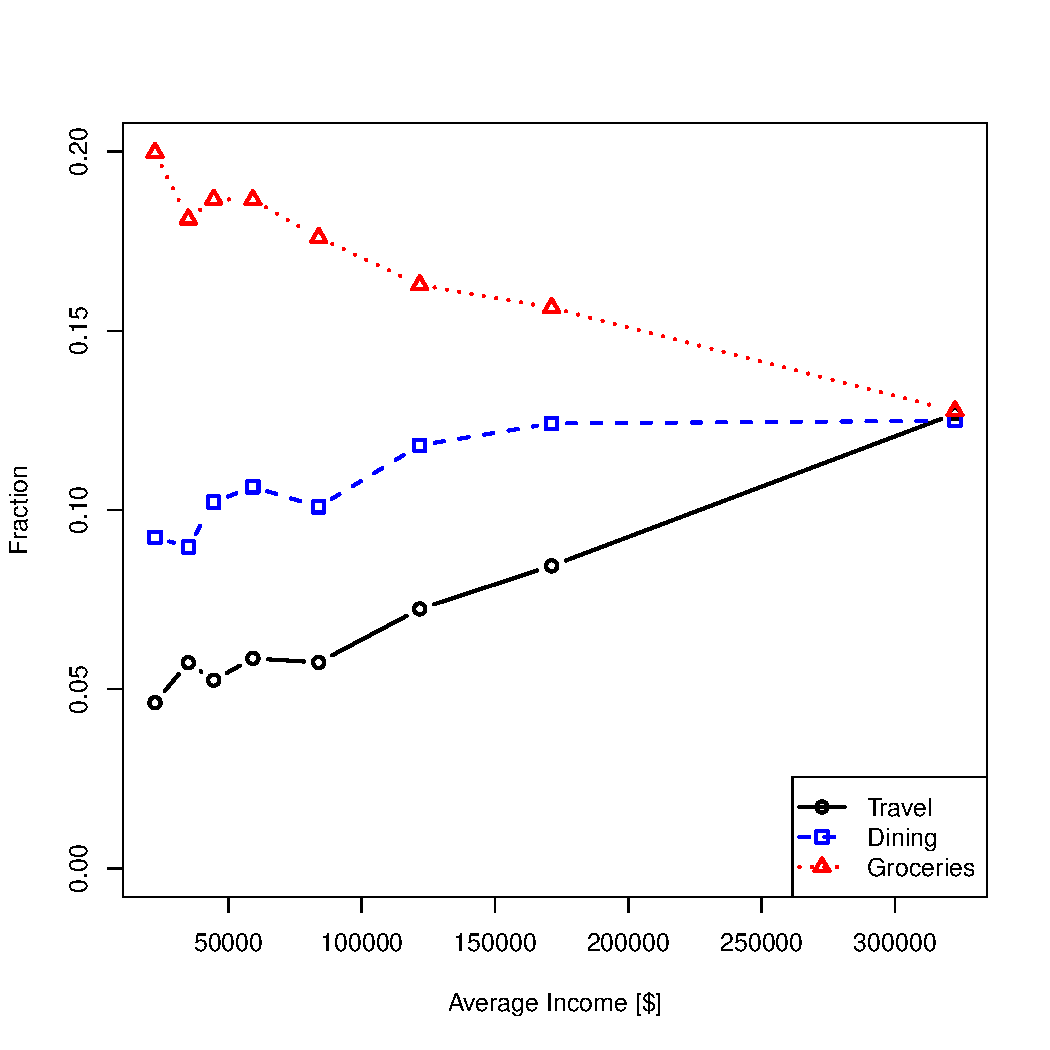
\includegraphics[width=0.6\textwidth]{../Figures/TravelDiningFraction.pdf}
    \caption{Fraction of total credit card spend going toward travel, dining, and groceries, for the average incomes from the BLS CES data (mapped to the credit card spending categories).}
    \label{fig:TravelDiningFraction}
    \end{center}
\end{figure}

Using a logarithmic scale for income, Fig.~\ref{fig:MC_ROS_vs_Income} shows a smoothed density scatterplot of all 100,000 simulated portfolios.  
This shows where the highest density of our ``observations'' are, as well as how ROS varies with income. 
Per income, the vertical spread in density is caused by the random sampling of $K$ (number of cards), $\eta$ (use of transfer partners), and $\theta$ (use of benefits).
The spread in the horizontal direction is caused by the observed Floridian income distribution.
A ``loess'' curve (short for ``locally estimated scatterplot smoothing'') is overplotted in red, and highlights a trend where the mean ROS is increasing for incomes above $\sim\$120,000$.
This upward trend must be attributed to shifts in spending patterns with income. 
Looking at the fraction of spend going toward the travel, dining, and groceries categories in Fig.~\ref{fig:TravelDiningFraction}, we see that essentials like groceries becomes a less important part of the budget as income increases.
Travel, on the other hand, takes up a larger fraction of the budget for higher incomes, while dining (away from home) shows this effect to a smaller degree. 
Not surprisingly, in our credit cards dataset we find some of the highest point multipliers on the travel categories, usually on cards with the highest annual fees, such as the American Express Platinum and the Chase Sapphire Reserve. 
High-income individuals can more easily justify these high annual fees, especially since they also have the spending behavior that matches well with the rewards categories of these cards, leading to above-average benefits.   

Finally, the results of the Monte Carlo simulation can be used to show how often a specific credit card ends up in a recommended portfolio. 
Figure~\ref{fig:MC_Popularity_100k} shows the top 10 most recommended cards. 
The Amazon Prime card and the American Express Blue Cash Preferred are the two most recommended cards, followed closely by the Wells Fargo Autograph.

\begin{figure}[t!bh]
    \begin{center}
    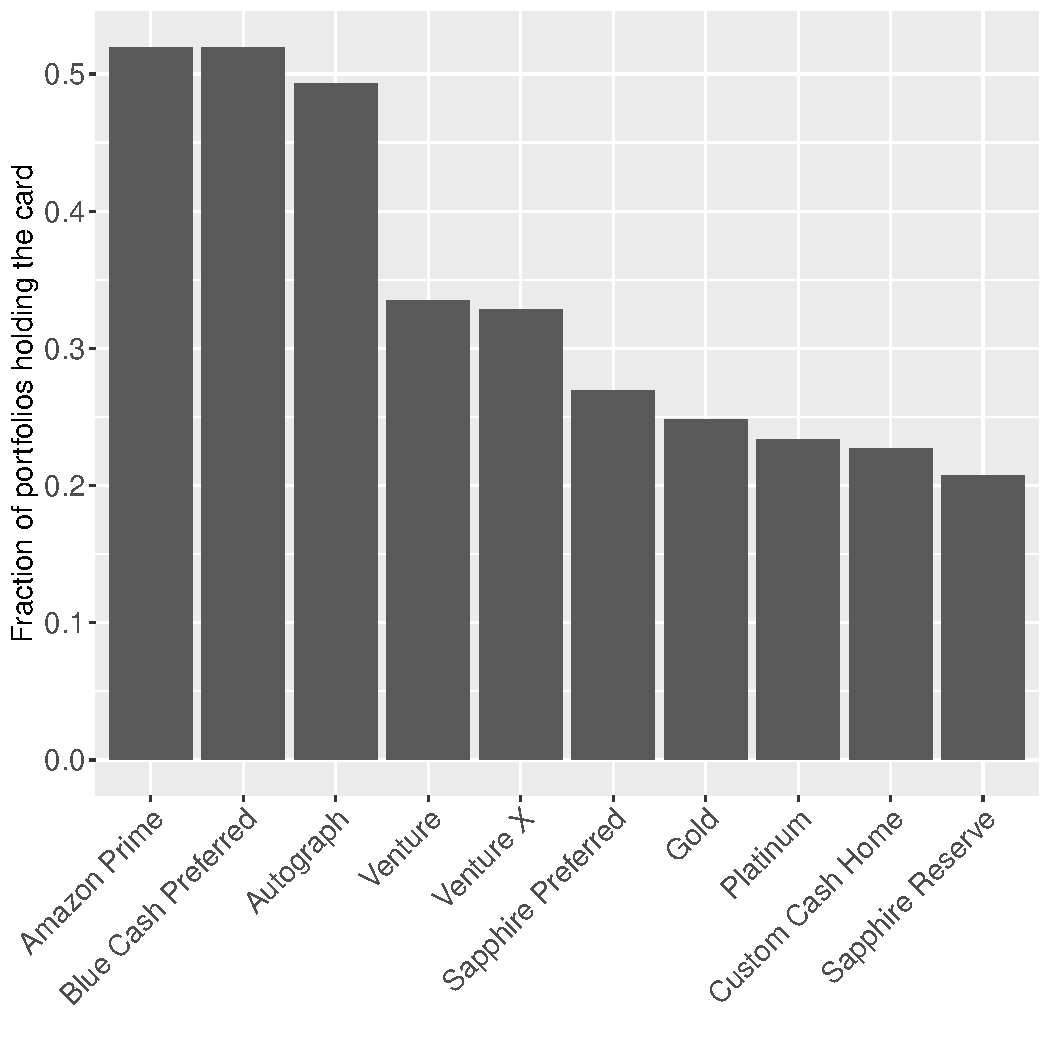
\includegraphics[width=0.7\textwidth]{../Figures/MC_Popularity_M100k.pdf}
    \caption{Top 10 most recommended credit cards from the Monte Carlo simulation.}
    \label{fig:MC_Popularity_100k}
    \end{center}
\end{figure}

\clearpage
\subsection{Shiny App} \label{subsec:ShinyApp}

No credit card user is the same. 
Above we have seen how credit card rewards can benefit users with average income levels and average budgets, but what we really need is a way to make \emph{personal} recommendations based on someones individual spending behavior, point valuations, and other preferences. 
This is why I have also developed an \sR\ \textsf{Shiny} app that will return the optimal portfolio for a user's personal preferences and individual budget.

A screenshot of the current version of the app is shown in Fig.~\ref{fig:REMCCO}, and the app can be accessed online at \url{https://remcoscheepmaker.shinyapps.io/ReMCCO/}.%
\footnote{The working title of the app is ``ReMCCO'', which stands for Recommend Me Credit Cards Optimally.}
Every \textsf{Shiny} app consists of a user interface and a server function. 
The server function makes use of exactly the same \texttt{get\_budget()} and \texttt{get\_portfolio()} functions as the rest of this project (presented in the Code Appendix), so the underlying algorithm works the same (although the app rounds the budget to the nearest dollar, which explains small differences between Figs.~\ref{fig:Waterfall} and \ref{fig:REMCCO}).

In the left column of the user interface, a user can specify preferences such as number of cards ($K$), use of transfer partners ($\eta$), use of benefits ($\theta$), and which banks to include. 
In a second column, the spending budget is pre-filled to match an average budget based on income (using Table~\ref{tab:BudgetIncome}), but the user can adjust this budget freely, either by adjusting the income, or by changing the amount for each category individually, making the budget completely personal. 
The waterfall plot in the top right will automatically adjust after each change (using \textsf{Shiny's} ``reactive'' programming functionality). 
This waterfall plot shows the recommended credit card portfolio, including the marginal and total benefits, just like Fig.~\ref{fig:Waterfall}. 
Underneath the figure some summary information is printed, and the card assignments are presented in a table (to show which card to use for each spending category).

In its current form, the app already has more functionality than what was captured by the variables and parameters that I used in the analysis above, since the user can also filter for banks and personalize the budget. 
The app could be further improved, however, by also making the valuations of points and benefits user-adjustable. 
This way, the user can specify that it values points or benefits from certain banks differently, for example because one bank has a transfer partner that the user really values, or because the user is a preferred client at one bank, which might come with additional benefits.%
\footnote{For example, Bank of America's \emph{Preferred Rewards} program offers 25, 50, or 75~percent higher point values for clients with \$20,000, \$50,000, or \$100,000 in combined assets at Bank of America / Merrill.} 
A future update of the app is planned to include these improvements. 

\begin{landscape}
\begin{figure}[t!h]
    \begin{center}
    \includegraphics[scale=0.45]{../Misc/REMCCO.png}
    \caption{Screenshot of the online \sR\ \textsf{Shiny} user interface at \url{https://remcoscheepmaker.shinyapps.io/ReMCCO/}.}
    \label{fig:REMCCO}
    \end{center}
\end{figure}
\end{landscape}

